% arara: latexmk: { engine: pdflatex, clean: partial }
% arara: clean: { extensions: [ptc,bbl,glsdefs,SAVE-ERROR,lol] }
% arara: pdflatex: { shell: yes, interaction: nonstopmode }
% arara: biber
% arara: pdflatex: { shell: yes, interaction: nonstopmode, synctex: yes }
% arara: pdflatex: { shell: yes, interaction: nonstopmode, synctex: on }
% arara: latexmk: { engine: pdflatex, clean: partial }
% arara: clean: { extensions: [ptc,bbl,glsdefs,SAVE-ERROR,lol] }
\documentclass[twoside,spanish,a4paper,12pt]{tfg}

% Editar la titulación
\titulacion{Grado en Ingeniería \\ Multimedia}

% Título del TFG (provisional)
\title{Plataforma web para el emparejamiento de profesionales y proyectos basada en competencias}

% Si es una alumna se debe usar
% \authorlabel{Autora}
\authorlabel{Autor}
% Editar el nombre
\author{Javier León Soler}


% Si hay varios tutores:
% \tutorlabel{Tutores}
% \tutor{Nombre del tutor 1 \\[2mm] Nombre del turor2}
% Si el tutor es masculino:
% \tutorlabel{Tutor}
\tutorlabel{Tutor}
% Editar
\tutor{Raúl Peña Ortiz}

% Editar: Poner mes y año de la convocatoria de lectura del TFM
\convocatoria{Julio 2025}

\addbibresource{references.bib}

\setcounter{secnumdepth}{4}

\makeatletter

\makenoidxglossaries
\loadglsentries{tex/acronimos-terminos}

\makeatletter

\begin{document}

% NO QUITAR ESTOS ELEMENTOS
\portada
\cleardoublepage
\contraportada
\cleardoublepage
\declaracion
\cleardoublepage


% Editar: Resumen en Español (obligatorio)
\begin{resumen}
  Este es el resumen de \gls{tfg}. Debe ser corto (máximo media página) y cubrir los aspectos principales del \gls{tfg}.
\end{resumen}
\cleardoublepage

% Editar: Resumen en Inglés
\begin{abstract}
  This is the abstract of the \gls{tfg}. It must be short and cover the main aspects of the \gls{tfg}.
\end{abstract}
\cleardoublepage

% Editar: Resumen en Valenciano
\begin{resum}
  Aquest és el resum del \gls{tfg}. Ha de ser curt (màxim mitja pàgina) i cobrir els aspectes principals del \gls{tfg}.
\end{resum}
\cleardoublepage


% Editar: Agradecimientos (opcional)
\begin{agradecimientos}
  En primer lugar quiero agradecer a todos aquellos que me han apoyado durante todos estos años.

  En segundo lugar...
\end{agradecimientos}
\cleardoublepage



\tableofcontents
\cleardoublepage
\listoffigures
\cleardoublepage
\listoftables
\cleardoublepage
\lstlistoflistings


\pagestyle{tfg}
\justify

% Las figuras se buscan en el directorio figs

% Cada capítulo está en su propio fichero tex. Ver el directorio tex.

% La bibliografía está dentro del directorio bib
\chapter{Introducción}
% Contenidos del capítulo.
% Las secciones presentadas son orientativas y no representan
% necesariamente la organización que debe tener este capítulo.

\section{Introducción}


\section{Motivación}


\section{Objetivos}


\section{Organización de la memoria}


\chapter{Estado del arte}\label{ch:estado-arte}
% Contenidos del capítulo.
% Las secciones presentadas son orientativas y no representan
% necesariamente la organización que debe tener este capítulo.

% Introducción
En el presente capítulo se lleva a cabo un análisis del estado del arte con el fin de situar el 
proyecto en el contexto de soluciones existentes y tecnologías actuales. La plataforma 
web desarrollada en este trabajo tiene como objetivo facilitar el emparejamiento entre 
profesionales y proyectos mediante un sistema basado en competencias jerarquizadas. 
Por ello, resulta esencial estudiar qué herramientas similares existen ya en el mercado 
y cómo se enfrentan a problemas de emparejamiento, recomendación o gestión de 
talento y proyectos.

Primero se presentarán aplicaciones con funcionalidades relacionadas, analizando sus 
características principales, puntos en común con esta propuesta y diferencias clave. 
Este estudio permitirá identificar tanto aspectos que se consideran imprescindibles en 
una plataforma de este tipo, como oportunidades de mejora o innovación.

Posteriormente se realizará un análisis crítico de las tecnologías más relevantes para el 
desarrollo del sistema, justificando la elección final en cada caso a partir de criterios 
como la escalabilidad, facilidad de desarrollo, mantenimiento o compatibilidad entre 
componentes.

Por último, se listarán aquellas herramientas de soporte utilizadas durante el desarrollo 
del trabajo, como entornos de desarrollo, sistemas de control de versiones o editores 
de diagramas, las cuales han sido fundamentales para llevar a cabo el proyecto.


\section{Análisis de aplicaciones similares}
% Qué aplicaciones similares hay y en qué se diferencia de ellas la propuesta
En esta sección se analizarán distintas aplicaciones existentes que presentan elementos 
comunes con la \textbf{plataforma web desarrollada en este trabajo}, cuyo objetivo es 
facilitar el \textbf{emparejamiento entre profesionales y proyectos} en función de sus 
competencias. Para ello, se comentarán \textbf{soluciones reales} que abordan problemas 
similares, ya sea desde la perspectiva de \textbf{plataformas orientadas al empleo y el talento}, 
o desde el enfoque de \textbf{sistemas de emparejamiento inteligente basados en afinidad}.

Dado que el proyecto combina ideas presentes en entornos profesionales como LinkedIn \cite{linkedin}
y en algoritmos de emparejamiento como los utilizados por aplicaciones tipo Tinder \cite{tinder}, se 
ha optado por dividir este análisis en \textbf{dos bloques diferenciados}. En el primero se 
estudiarán \textbf{plataformas centradas en la gestión del talento y la búsqueda de empleo}, 
mientras que en el segundo se abordarán \textbf{sistemas cuyo núcleo es el emparejamiento 
basado en coincidencias}, con el objetivo de extraer ideas aplicables al 
\gls{recomendaciones} que se desea implementar.

Este análisis permitirá no solo \textbf{identificar funcionalidades clave y enfoques existentes}, 
sino también detectar \textbf{carencias o posibles áreas de mejora}, con el fin de proponer 
una solución más \textbf{adaptada, automatizada} y centrada en la 
\textbf{coincidencia de competencias concretas}.

\subsection{Plataformas web orientadas al empleo y la gestión del talento}

Dado que la plataforma web a desarrollar tiene como objetivo conectar profesionales con 
proyectos en función de sus competencias, las primeras aplicaciones a analizar son aquellas 
centradas en la búsqueda de empleo, la exposición del perfil profesional y la gestión del talento.

En esta sección se analizarán concretamente las plataformas \textbf{LinkedIn} \cite{linkedin}, 
\textbf{InfoJobs} \cite{infojobs} y \textbf{Yobalia} \cite{yobalia}, destacando sus funcionalidades principales y su grado 
de similitud con la solución propuesta en este trabajo.

\subsubsection{LinkedIn}
LinkedIn es una de las plataformas más conocidas y utilizadas a nivel mundial...


\subsection{Aplicaciones con sistemas de emparejamiento basados en coincidencias}


\section{Evaluación de tecnologías}\label{sec:evaluacion-tecnologias}
% Análisis crítico de las tecnologías y sistemas de despliegue posibles y por qué se han seleccionado unas concretas.


\chapter{Requisitos, especificaciones, planificación, coste, riesgos y viabilidad}\label{ch:requisitos}
% Contenidos del capítulo
%Las secciones presentadas son orientativas y no representan necesariamente la organización que debe tener este capítulo.

\section{Requisitos}

\subsection{Requisitos funcionales}

\subsection{Requisitos no funcionales}

Se debe optar por formular los requisitos de forma que se pueda
conocer si se han alcanzado o no a la finalización del proyecto. Por
ejemplo, es difícil valorar si el siguiente requisito funcional se
alcanza o no: \textit{El sistema debe retornar una respuesta en un tiempo
razonable cuando tenga muchos usuarios concurrentes}. ¿Cuánto es un
tiempo razonable?, ¿cuantos son muchos usuarios?. Sin embargo, si se
formula de este otro modo: \textit{El sistema debe retornar una
respuesta en menos de un segundo cuando tenga 200 usuarios
concurrentes}, es fácil comprobar si se ha alcanzado ejecutando un
plan de pruebas, por ejemplo con JMeter.

\section{Especificaciones}\label{sec:especificaciones-sistema}
Especificación del proyecto a partir de los requisitos.
Una vez se han definido los requisitos funcionales y no funcionales del sistema, se procede a especificar el sistema a partir de ellos. En este apartado se muestan características del sistema, sin entrar en detalles de diseño e implementación, que permiten entender el problema al que nos enfrentamos pero no como lo vamos a afrontar (etapa de diseño).
Se recomienda confeccionar una arquitectura de referencia, o imagen no técnica (más bien comercial) que ilustre los actores y aplicaciones principales que conforman el sistema.

\section{Planificación y estimación de costes}
Describir el tipo de metodología de desarrollo que se va a utilizar
(cascada, ágil, etc).
Tareas a realizar, estimación de la duración de las tareas, y
distribución temporal (por ejemplo con un diagrama de Gantt).

Enumerar las tareas a realizar, estimación de la duración de las tareas, y
distribución temporal (por ejemplo con un diagrama de Gantt).

Costes de personal (teniendo en cuenta los costes de seguridad
social), de hardware (imputando solo la duración del proyecto y teniendo
en cuenta que los equipos se amortizan en 3 o 4 años) y/o de software.
Además, hay que añadir costes indirectos.

\section{Riesgos}

Identificación de los riesgos que pueden aparecer durante el
desarrollo del proyecto, su probabilidad de ocurrencia, su impacto en
el proyecto y las medidas que se podrían adoptar para mitigarlos.

\section{Viabilidad}
En este apartado, dependiendo de la naturaleza del proyecto, se
debería analizar la viabilidad técnica y la viabilidad económica. Para
la viabilidad técnica hay que analizar si los recursos
necesarios (herramientas, conocimientos, experiencia, etc)  para llevar
a cabo el proyecto permiten realizarlo en el tiempo previsto.
En cuanto a la viabilidad económica hay que evaluar si el proyecto
será rentable cuando esté operativo.

\chapter{Análisis}
% Contenidos del capítulo.
% Las secciones presentadas son orientativas y no representan
% necesariamente la organización que debe tener este capítulo.

\section{Diagrama de casos de uso}

Identificación de actores y diagramas de casos de uso asociados a los requisitos funcionales.

\section{Diagrama de secuencia}
Para los casos de uso más importantes y complejos se deben especificar los diagramas de secuencia que describan el comportamiento de los objetos que intervienen en el caso de uso.
\section{Diagrama de clases de primer nivel}

Al final del análisis se debe presentar un diagrama de clases de primer nivel que muestre las clases principales del sistema y sus relaciones.
Para cada una de las clases que tengan un estado complejo o relevante, se debe especificar el diagrama de estados asociado o el diagrama de actividades en el que se involucra la clase.

\chapter{Diseño}
% Contenidos del capítulo.
% Las secciones presentadas son orientativas y no representan
% necesariamente la organización que debe tener este capítulo.

% Diagramas de clases, de secuencia, de despliegue, diseño de
% pantallas, etc

\section{Arquitectura de componentes}

A partir de la especificación realizada en la sección \ref{sec:especificaciones-sistema} del Capítulo \ref{ch:requisitos} y la tecnología seleccionada en la sección \ref{sec:evaluacion-tecnologias} del Capítulo \ref{ch:estado-arte}, se debe construir el diagrama de componentes UML que represente la arquitectura de referencia del sistema. 
En este diagrama se deben identificar los componentes principales del sistema y las relaciones entre ellos, pasando a detallar los subcomponentes de cada uno de ellos en secciones posteriores.

\section{Despliegue del sistema}

En esta sección se debe presentar el diagrama de despliegue del sistema, que muestre la arquitectura física del sistema y cómo se distribuyen los componentes en los nodos físicos o virtuales que lo componen.
En otras palabras, para cada componente principal del sistema se identifica en que servidor físico o virtual se va a ejecutar.

Se puede definir un despligue de desarrollo (el despliegue que se tiene en el portátil mientras se trabaja), uno de producción (despliegue final o real) y uno de pruebas (lo más parecido posible al real).

\section{Modelo de datos}

En este caso se puede especificar el diagrama de clases final del diseño atendiendo al lenguaje de programación y a la tecnología seleccionada.
Además será necesario, como mínimo, especificar el modelo físico de datos, en el lenguaje SQL propio de la base de datos relacional seleccionada, o el modelo de documentos, si se utiliza una base de datos NoSQL. 


\chapter{Implementación y pruebas}
% Contenidos del capítulo.
% Las secciones presentadas son orientativas y no representan
% necesariamente la organización que debe tener este capítulo.
Las secciones presentadas son orientativas y no representan
necesariamente la organización que debe tener este capítulo.
\section{Implementación}
Presentar cómo se ha organizado el desarrollo de los proyectos
(capturas del IDE), trozos de código relevantes, cómo han quedado
implementadas las interfaces gráficas de usuario, etc.
\section{Pruebas unitarias}
Descripción de las pruebas que se han llevado a cabo para comprobar que el código
desarrollado es correcto (JUnit, etc).
\section{Pruebas funcionales}
Descripción de las pruebas que se han llevado a cabo para comprobar que los casos de uso
identificados funcionan correctamente.
\section{Pruebas de rendimiento}
Descripción de las pruebas de estrés realizadas para comprobar los tiempos de
respuesta de la aplicación (según figuren en los requisitos).
\section{Pruebas de usabilidad}
Descripción de las pruebas que se han llevado a cabo con usuarios para determinar el
nivel de usabilidad de la aplicación (que se hayan recogido en los requisitos).
\section{Pruebas de seguridad}
Descripción de las pruebas realizadas para comprobar que se cumplen las
restricciones de autenticación y de autorización que se han descrito
en los requisitos.

\chapter{Conclusiones}
% Contenidos del capítulo.
% Las secciones presentadas son orientativas y no representan
% necesariamente la organización que debe tener este capítulo.

\section{Revisión de costes}

Al finalizar el proyecto hay que ver en qué fases de la ejecución nos
hemos desviado, explicar los motivos y calcular el coste real con
estos ajustes.

\section{Conclusiones}

\section{Trabajo futuro}


\printbibliography[heading=bibnumbered, title={Bibliografía \label{chap:bibliography}}]


\pagestyle{appendix}

\appendix

\chapter{Glosarios}
%\addcontentsline{toc}{chapter}{Acrónimos}
%\printnoidxglossary[type=\acronymtype, title=Acrónimos y abreviaciones, toctitle=Acrónimos y abreviaciones]
\printnoidxglossary[type=\acronymtype, title=Acrónimos y abreviaciones]

%\section{Términos}

\printnoidxglossary[type=main,title=Términos]
%\addcontentsline{toc}{chapter}{Glosario}
%\printnoidxglossary[type=main,title=Términos, toctitle=Términos]

\chapter{Ejemplos del lenguaje de marcado \LaTeX{}}

\section{Algunos ejemplos básicos de uso de \LaTeX{}}

  \textbf{Texto} en el párrafo 1.

  \textit{Texto} en el párrafo 2.

  \texttt{Texto} en el párrafo 3.


  \begin{itemize}
  \item Consideración 1
  \item Consideración 2
  \end{itemize}

  % Espacio vertical
  \vspace{0.5cm}
  
  \begin{enumerate}
  \item Punto 1
  \item Punto 2
  \end{enumerate}
  
A continuación se muestra una ecuación:

  \[ \int_{0}^{1}\frac{1}{x^2+1} dx \]

  \section{Figuras y subfiguras}

  Podemos incluir imágenes en formato: png, pdf o jpg.

  En la Figura~\ref{fig:diagrama} se muestra un diagrama\footnote{Realizado con \href{yed}{https://www.yworks.com/products/yed}}, mientras que la Figura~\ref{fig:diagramas} muestra varios diagramas en mosaico, de manera que puedo referirme al segundo diagrama como Figura~\ref{fig:diagrama-2}.

  \begin{figure}[!htb]
    \centering
    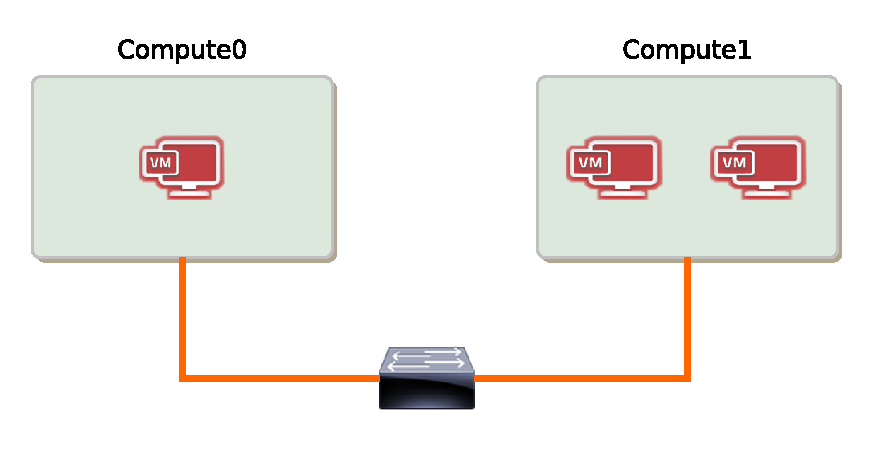
\includegraphics[width=0.8\textwidth]{diagrama.pdf}
    \caption{Esta es una figura que latex decide donde colocar (floating) en el documento.}
    \label{fig:diagrama}
  \end{figure}

  \begin{figure}[h!t]
    \centering
    \begin{subfigure}{0.45\textwidth}
        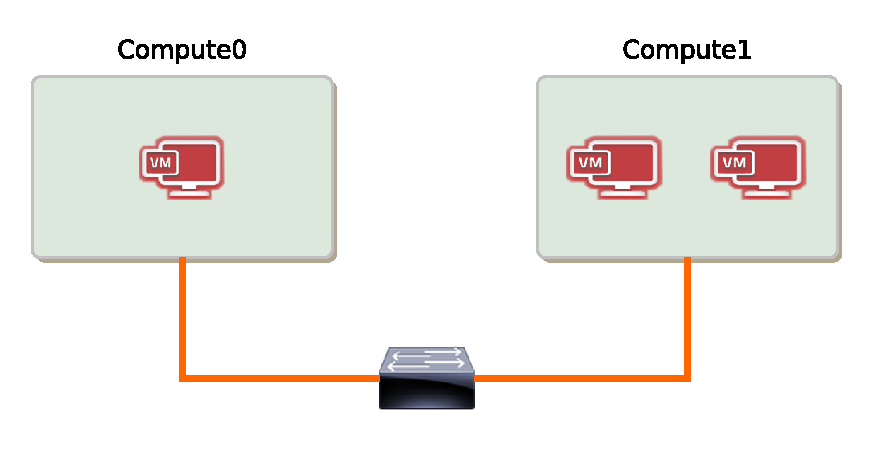
\includegraphics[width=\textwidth]{diagrama.pdf}
        \caption{Copia 1}\label{fig:diagrama-1}
    \end{subfigure}
    \hfill
    \begin{subfigure}{0.45\textwidth}
        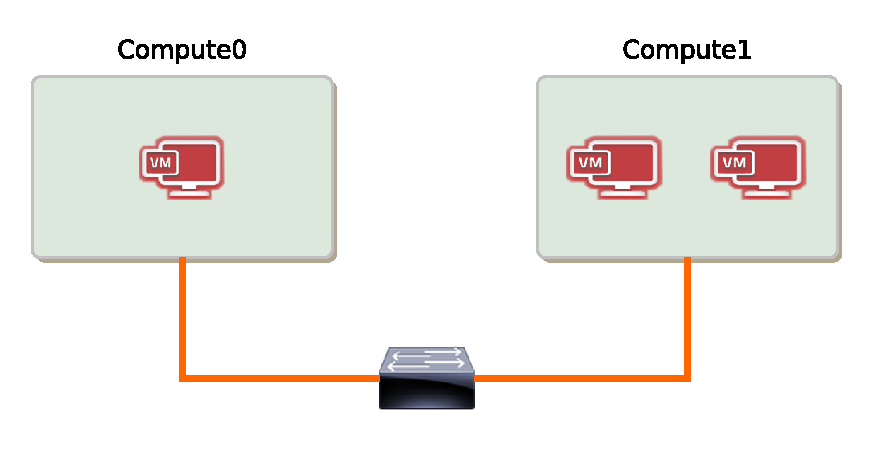
\includegraphics[width=\textwidth]{diagrama.pdf}
        \caption{Copia 2}\label{fig:diagrama-2}
    \end{subfigure}
    \vskip\baselineskip
    \begin{subfigure}{0.45\textwidth}
        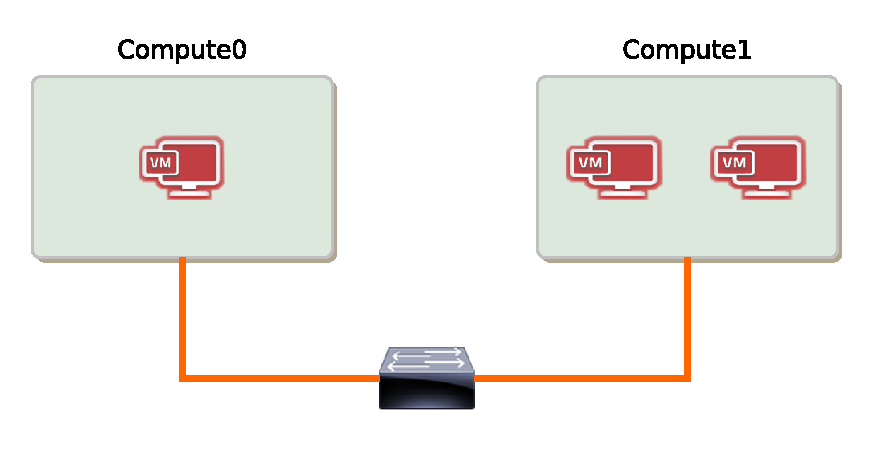
\includegraphics[width=\textwidth]{diagrama.pdf}
        \caption{Copia 3}\label{fig:diagrama-3}
    \end{subfigure}
    \hfill
    \begin{subfigure}{0.45\textwidth}
        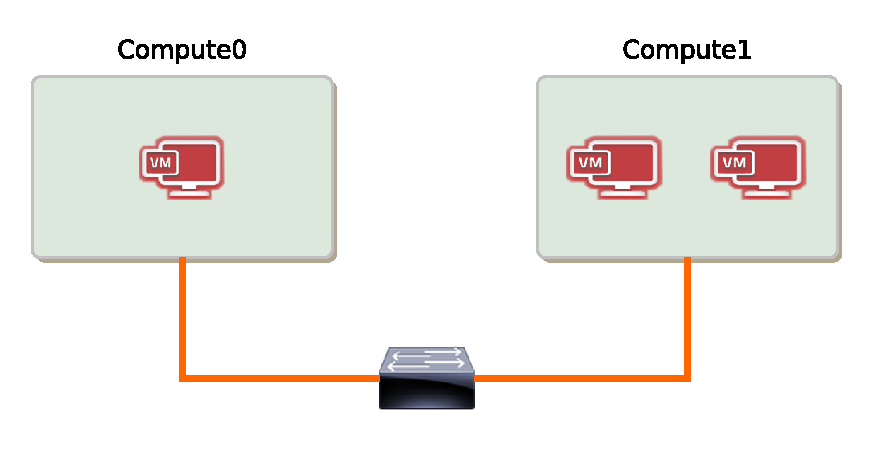
\includegraphics[width=\textwidth]{diagrama.pdf}
        \caption{Copia 4}\label{fig:diagrama-4}
    \end{subfigure}
    \caption{Los cuatro diagramas en mosaico}
    \label{fig:diagramas}
\end{figure}

\section{Tablas}
  
  La Tabla \ref{tab:ejemplo-1} es un ejemplo de una tabla.
  
  \begin{table}[!htb]
    \centering
  \begin{tabular}{|l|c|}
    \hline
    Columna 1 & Columna 2 \\ \hline
    1 & 2 \\ \hline
  \end{tabular}
  \caption{Ejemplo de tabla 1}
  \label{tab:ejemplo-1}
\end{table}

  Existen también tablas más complejas que requieren un mayor control de la posición de los elementos, como la Tabla \ref{tbl:phd-raul} que ha sido extraída de \cite{rpo:tesis-2013}, o de varias páginas, como la Tabla~\ref{tab:long}. 

  \begin{sidewaystable}
    \centering
    \begin{tabular}{|l|c|c|c|c|c||c|c|c||c|c|c|c|c|c|c|c|c|c|}
    \cline{2-17}
    \cline{2-17}
    \multicolumn{1}{l|}{} & \multicolumn{5}{c||}{GROUP I} & \multicolumn{3}{c||}{GROUP II} &
    \multicolumn{8}{c|}{GROUP III}\\
    \cline{2-17}
    \hline
    
    \backslashbox[60mm]{FEATU./CAPAB.}{GENERATOR}
    &
    % Benchmarks
    \begin{sideways}WebStone\end{sideways}&
    \begin{sideways}SPECweb\end{sideways} &
    \begin{sideways}SURGE\end{sideways} &
    \begin{sideways}Web Polygraph\end{sideways} &
    \begin{sideways}TPC-W\end{sideways} &
    
    % Grupo de generadores de carga que producen dinamismo
    \begin{sideways}LoadRunner\end{sideways} &
    \begin{sideways}WebLOAD\end{sideways} &
    \begin{sideways}JMeter\end{sideways} &
          
    % Herramientas para la generación de carga
    \begin{sideways}S-Clients\end{sideways} &
    \begin{sideways}WebJamma\end{sideways} &
    \begin{sideways}Deluge\end{sideways} &
    \begin{sideways}HAMMERHEAD 2\hspace{0.25cm} \end{sideways} &
    \begin{sideways}PTester\end{sideways} &
    \begin{sideways}Siege\end{sideways} &
    \begin{sideways}HTTPERF \end{sideways} &
    \begin{sideways}Autobench\end{sideways}\\
    
    \hline\color{black}\scriptsize{Analytical-Based
    Architecture}& {\color{gray}\faStar{}} & {\color{gray}\faStar{}} &
    {\color{gray}\faStar{}} & {\color{gray}\faStar{}} & {\color{gray}\faStar{}} & {\color{gray}\faStarHalf*{}}& {\color{gray}\faStarHalf*{}}& {\color{gray}\faStarHalf*{}}& & & & &
    & & & \\
    
    \hline\scriptsize{Distributed Architecture}& {\color{gray}\faStar{}} &
    {\color{gray}\faStar{}} & {\color{gray}\faStar{}} &  {\color{gray}\faStar{}} & & {\color{gray}\faStar{}} & {\color{gray}\faStar{}} &  &  &  &  &  &  &
     &  & \\
    
    \hline\scriptsize{Business-Based Architecture} & & {\color{gray}\faStarHalf*{}} & & {\color{gray}\faStarHalf*{}} & {\color{gray}\faStar{}} & {\color{gray}\faStar{}} & {\color{gray}\faStar{}} & {\color{gray}\faStar{}} & & & & & & & & \\
    
    \hline\scriptsize{Client Parameterization} & {\color{gray}\faStar{}} &
    {\color{gray}\faStar{}} & & {\color{gray}\faStarHalf*{}} & {\color{gray}\faStar{}} & {\color{gray}\faStar{}} & {\color{gray}\faStar{}} & {\color{gray}\faStar{}} & & {\color{gray}\faStar{}} & & {\color{gray}\faStarHalf*{}} & & & {\color{gray}\faStarHalf*{}} &  \\
    
    \hline\scriptsize{Workload Types} & & {\color{gray}\faStar{}} & & & {\color{gray}\faStar{}} & {\color{gray}\faStar{}} &{\color{gray}\faStar{}}  & {\color{gray}\faStarHalf*{}}
    & & & & & & & & \\
    
    \hline\scriptsize{Functional Testing} & & & & & & {\color{gray}\faStar{}} &{\color{gray}\faStar{}} &  {\color{gray}\faStarHalf*{}} & & & &{\color{gray}\faStarHalf*{}} &{\color{gray}\faStarHalf*{}}
     &{\color{gray}\faStarHalf*{}} & & {\color{gray}\faStarHalf*{}}\\
    
    \hline\scriptsize{LAN and WAN}& & & & & & & & & {\color{gray}\faStar{}} & & &
    & & & & \\
    
    \hline\scriptsize{Multi-platform}&{\color{gray}\faStar{}}&{\color{gray}
    \faStar{}}&{\color{gray}\faStar{}}&{\color{gray}\faStar{}}&{
    \color{gray}\faStar{}}&{\color{gray}\faStar{}}&{\color{gray}\faStar{}}&{\color{gray}\faStar{}}&{\color{gray}\faStar{}}&{\color{gray}\faStar{}}&{\color{gray}\faStar{}}&{\color{gray}\faStarHalf*{}}&{\color{gray}\faStar{}}&{\color{gray}\faStarHalf*{}}&{\color{gray}\faStar{}}&{\color{gray}\faStar{}}\\
    
    \hline\scriptsize{Ease of Use}& & & & & &{\color{gray}\faStar{}} &{\color{gray}\faStar{}} & {\color{gray}\faStarHalf*{}} & & & & & & & &\\
    
    \hline\scriptsize{Performance Reports} &  
    {\color{gray}\faStarHalf*{}}& 
    {\color{gray}\faStar{}}&&
    {\color{gray}\faStar{}}&
    {\color{gray}\faStar{}}&
    {\color{gray}\faStar{}}&
    {\color{gray}\faStar{}}&
    {\color{gray}\faStar{}}&&&
    {\color{gray}\faStarHalf*{}}&
    {\color{gray}\faStarHalf*{}}&
    {\color{gray}\faStarHalf*{}}&
    {\color{gray}\faStarHalf*{}}&
    {\color{gray}\faStarHalf*{}}&
    {\color{gray}\faStarHalf*{}}\\
    
    \hline\scriptsize{Open Source}& 
    {\color{gray}\faStar{}}&&
    {\color{gray}\faStar{}}& 
    {\color{gray}\faStarHalf*{}}&
    {\color{gray}\faStar{}}&&&
    {\color{gray}\faStarHalf*{}}&
    {\color{gray}\faStar{}}&
    {\color{gray}\faStar{}}&
    {\color{gray}\faStar{}}& 
    {\color{gray}\faStar{}}&
    {\color{gray}\faStar{}}&
    {\color{gray}\faStar{}}&
    {\color{gray}\faStar{}}& 
    {\color{gray}\faStar{}}\\
    
    \hline
    \hline\rowcolor{dark-gray} {\color{black}\scriptsize{\textbf{User's Dynamism}}}& &
    & & & {\color{black}\faStarHalf*{}}
    &{\color{black}\faStarHalf*{}} & {\color{black}\faStarHalf*{}} &
    {\color{black}\faStarHalf*{}} & & & & & & & &\\
    
    \hline
    
    \end{tabular}
    \vspace{0.3cm}
    
    \begin{tabular}{ccc}
    \faStar{}  Full support & \faStarHalf*{} Partial support
    \end{tabular}
    
    \caption{Web workload generators and grade in which main features are
    fulfilled}\label{tbl:phd-raul}
    
    \end{sidewaystable}

  \begin{longtable}{|l|l|l|}
    \caption{Ejemplo de tabla muy larga para una página} \label{tab:long} \\
    
    \hline \multicolumn{1}{|c|}{\textbf{First column}} & \multicolumn{1}{c|}{\textbf{Second column}} & \multicolumn{1}{c|}{\textbf{Third column}} \\ \hline 
    \endfirsthead
    
    \multicolumn{3}{c}%
    {{\bfseries \tablename\ \thetable{} -- continued from previous page}} \\
    \hline \multicolumn{1}{|c|}{\textbf{First column}} & \multicolumn{1}{c|}{\textbf{Second column}} & \multicolumn{1}{c|}{\textbf{Third column}} \\ \hline 
    \endhead
    
    \hline \multicolumn{3}{|r|}{{Continúa en la siguiente página ...}} \\ \hline
    \endfoot
    
    \hline \hline
    \endlastfoot
    
    One & abcdef ghjijklmn & 123.456778 \\
    One & abcdef ghjijklmn & 123.456778 \\
    One & abcdef ghjijklmn & 123.456778 \\
    One & abcdef ghjijklmn & 123.456778 \\
    One & abcdef ghjijklmn & 123.456778 \\
    One & abcdef ghjijklmn & 123.456778 \\
    One & abcdef ghjijklmn & 123.456778 \\
    One & abcdef ghjijklmn & 123.456778 \\
    One & abcdef ghjijklmn & 123.456778 \\
    One & abcdef ghjijklmn & 123.456778 \\
    One & abcdef ghjijklmn & 123.456778 \\
    One & abcdef ghjijklmn & 123.456778 \\
    One & abcdef ghjijklmn & 123.456778 \\
    One & abcdef ghjijklmn & 123.456778 \\
    One & abcdef ghjijklmn & 123.456778 \\
    One & abcdef ghjijklmn & 123.456778 \\
    One & abcdef ghjijklmn & 123.456778 \\
    One & abcdef ghjijklmn & 123.456778 \\
    One & abcdef ghjijklmn & 123.456778 \\
    One & abcdef ghjijklmn & 123.456778 \\
    One & abcdef ghjijklmn & 123.456778 \\
    One & abcdef ghjijklmn & 123.456778 \\
    One & abcdef ghjijklmn & 123.456778 \\
    One & abcdef ghjijklmn & 123.456778 \\
    One & abcdef ghjijklmn & 123.456778 \\
    One & abcdef ghjijklmn & 123.456778 \\
    One & abcdef ghjijklmn & 123.456778 \\
    One & abcdef ghjijklmn & 123.456778 \\
    One & abcdef ghjijklmn & 123.456778 \\
    One & abcdef ghjijklmn & 123.456778 \\
    One & abcdef ghjijklmn & 123.456778 \\
    One & abcdef ghjijklmn & 123.456778 \\
    One & abcdef ghjijklmn & 123.456778 \\
    One & abcdef ghjijklmn & 123.456778 \\
    One & abcdef ghjijklmn & 123.456778 \\
    One & abcdef ghjijklmn & 123.456778 \\
    One & abcdef ghjijklmn & 123.456778 \\
    One & abcdef ghjijklmn & 123.456778 \\
    One & abcdef ghjijklmn & 123.456778 \\
    One & abcdef ghjijklmn & 123.456778 \\
    One & abcdef ghjijklmn & 123.456778 \\
    One & abcdef ghjijklmn & 123.456778 \\
    One & abcdef ghjijklmn & 123.456778 \\
    One & abcdef ghjijklmn & 123.456778 \\
    One & abcdef ghjijklmn & 123.456778 \\
    One & abcdef ghjijklmn & 123.456778 \\
    One & abcdef ghjijklmn & 123.456778 \\
    One & abcdef ghjijklmn & 123.456778 \\
    One & abcdef ghjijklmn & 123.456778 \\
    One & abcdef ghjijklmn & 123.456778 \\
    One & abcdef ghjijklmn & 123.456778 \\
    One & abcdef ghjijklmn & 123.456778 \\
    One & abcdef ghjijklmn & 123.456778 \\
    One & abcdef ghjijklmn & 123.456778 \\
    One & abcdef ghjijklmn & 123.456778 \\
    One & abcdef ghjijklmn & 123.456778 \\
    One & abcdef ghjijklmn & 123.456778 \\
    One & abcdef ghjijklmn & 123.456778 \\
    One & abcdef ghjijklmn & 123.456778 \\
    One & abcdef ghjijklmn & 123.456778 \\
    One & abcdef ghjijklmn & 123.456778 \\
    One & abcdef ghjijklmn & 123.456778 \\
    One & abcdef ghjijklmn & 123.456778 \\
    One & abcdef ghjijklmn & 123.456778 \\
    One & abcdef ghjijklmn & 123.456778 \\
    One & abcdef ghjijklmn & 123.456778 \\
    One & abcdef ghjijklmn & 123.456778 \\
    One & abcdef ghjijklmn & 123.456778 \\
    One & abcdef ghjijklmn & 123.456778 \\
    One & abcdef ghjijklmn & 123.456778 \\
    One & abcdef ghjijklmn & 123.456778 \\
    One & abcdef ghjijklmn & 123.456778 \\
    One & abcdef ghjijklmn & 123.456778 \\
    One & abcdef ghjijklmn & 123.456778 \\
    One & abcdef ghjijklmn & 123.456778 \\
    One & abcdef ghjijklmn & 123.456778 \\
    One & abcdef ghjijklmn & 123.456778 \\
    One & abcdef ghjijklmn & 123.456778 \\
    One & abcdef ghjijklmn & 123.456778 \\
    One & abcdef ghjijklmn & 123.456778 \\
    \end{longtable}
  
  \section{Listados}
  
  Para generar el fichero PDF, podemos usar los comandos del Listado \ref{lst:ejemplo-listado-bash}.
  
  \begin{listing}[!htb]
    \begin{minted}{bash}
      pdflatex main.tex
      bibtex main
      pdflatex main.tex
    \end{minted}
    \vspace*{-1cm}
    \captionsetup{type=lstlisting}
    \caption{Comandos bash para generar el fichero PDF}
    \label{lst:ejemplo-listado-bash}
  \end{listing}

  También se puede usar \texttt{arara} que automáticamente regenera la bibliografía, ver los comandos del Listado \ref{lst:ejemplo-listado-bash-2}.

  \begin{listing}[!htb]
    \begin{minted}{bash}
      arara main.tex
    \end{minted}
    \vspace*{-1cm}
    \captionsetup{type=lstlisting}
    \caption{Comandos bash para generar el fichero PDF con arara}
    \label{lst:ejemplo-listado-bash-2}
  \end{listing}

  También se pueden incluir listados de otros lenguajes como Python, ver Listado \ref{lst:python}, Java, ver Listado \ref{lst:java}, HTML\faHtml5{}, ver  Listado \ref{lst:html} o CSS\faCss3*{}, ver Listado \ref{lst:css}.

  \begin{listing}[!htb]
    \begin{minted}{python}
      def hello():
          print("Hello World!")
    \end{minted}
    \vspace*{-1cm}
    \captionsetup{type=lstlisting}
    \caption{Ejemplo de listado en Python}
    \label{lst:python}
  \end{listing}

  \begin{listing}[!htb]
    \begin{minted}{java}
      public class HelloWorld {
          public static void main(String[] args) {
              System.out.println("Hello, World");
          }
      }
    \end{minted}
    \vspace*{-1cm}
    \captionsetup{type=lstlisting}
    \caption{Ejemplo de listado en Java}
    \label{lst:java}
  \end{listing}

  \begin{listing}[!htb]
    \begin{minted}{html}
      <!DOCTYPE html>
      <html>
      <head>
      <title>Page Title</title>
      </head>
      <body>
      
      <h1>This is a Heading</h1>
      <p>This is a paragraph.</p>
      
      </body>
      </html>
    \end{minted}
    \vspace*{-1cm}
    \captionsetup{type=lstlisting}
    \caption{Ejemplo de listado en HTML\faHtml5{}}
    \label{lst:html}
  \end{listing}

  \begin{listing}[!htb]
    \begin{minted}{css}
      body {
          background-color: lightblue;
      }
      
      h1 {
          color: white;
          text-align: center;
      }
      
      p {
          font-family: verdana;
          font-size: 20px;
      }
    \end{minted}
    \vspace*{-1cm}
    \captionsetup{type=lstlisting}
    \caption{Ejemplo de listado en CSS\faCss3*{}}
    \label{lst:css}
  \end{listing}

  
  \section{Acrónimos y términos}

  \LaTeX{} tiene un paquete de glosario de términos y acrónimos que permite definir términos y acrónimos y usarlos en el texto.
  Lo que al principio puede parecer engorroso, una vez se usa, es muy útil.
  
  Usamos por primera vez el acrónimo \gls{tfm} y luego volvemos a usar el acrónimo \gls{tfm}, que ahora aparece abreviado, y por primera vez el término \gls{middleware}.
  
  Tenemos una opción especial para la forma plural de los acrónimos, como \glspl{sgbd}, aunque luego se usen en singular, \gls{sgbd}.
  
  Podemos forzar que aparezca el término completo, \glsentrylong{tfg}, abreviado, \glsentryshort{tfg}, o ambos, \glsentryfull{tfg}.
  Aunque en estos casos no nos lleva a la tabla de acrónimos y términos.
  
  El fichero {\tt acronimos-terminos.tex} contiene ejemplos de definición de acrónimos y términos.

  \chapter{Ejemplos de uso de \BibTeX{} como gestor de bibliografia}

Este apéndice muestra ejemplos de uso de \BibTeX{} como gestor de bibliografia.

\section{Ejemplos de referencias formales bien valoradas}

\begin{itemize}
  \item Un libro \cite{libro} o un capítulo de libro \cite{capitulo}.
  \item Un artículo de revista \cite{articulo}.
  \item Una publicación en una conferencia \cite{conferencia} o una publicación de conferencia que forma parte de una colección \cite{coleccion}.
  \item Una tesis doctoral \cite{tesis}.
  \item Un informe técnico específico del NIST \cite{informe-especifico}.
\end{itemize}

\section{Ejemplos de referencias con valoración intermedia}

\begin{itemize}
  \item Un informe técnico genérico \cite{informe}.
  \item Un \gls{tfg} \cite{tfg} o un \gls{tfm} \cite{tfm}.
\end{itemize}

\section{Ejemplos de referencias con valoración baja a evitar en la medida de lo posible}
\begin{itemize}
  \item Un manual online \cite{manual}.
  \item Una página web \cite{website}.
\end{itemize}

\end{document}

%%% Local Variables:
%%% mode: latex
%%% TeX-master: t
%%% End:
